%By Liping Wang at 2019-09-21
%Contact wangliping2019@ia.ac.cn
\documentclass{article}
\usepackage[UTF8]{ctex}
\usepackage{amsmath}
\usepackage{hyperref}
\usepackage{fancyhdr}
\usepackage{bbm}
\usepackage{graphicx}
\usepackage{url}
\usepackage{algorithm}
\usepackage[noend]{algpseudocode}

\topmargin=-0.45in
\evensidemargin=0in
\oddsidemargin=0in
\textwidth=6.5in
\textheight=9.0in
\headsep=0.25in
\linespread{1.1}



%配置区
\newcommand{\courseName}{算法设计与分析}
\newcommand{\homeworkId}{\#5} %作业编号
\newcommand{\homeworkTitle}{作业\homeworkId}
\newcommand{\studentId}{201928015059003}%学号
\newcommand{\studentName}{杨天健}%姓名


\newcommand{\question}[1]{\section*{Question #1}}
\renewcommand{\part}[1]{\subsection*{(#1)}}



\pagestyle{fancy}
\lhead{\studentName}
\rhead{\courseName\homeworkTitle}
\cfoot{\thepage}

\title{
    \vspace{2in}
    \textmd{\textbf{\courseName}:\homeworkTitle}\\
    \vspace{0.1in}
    \large{\studentId}\\
    \large{\studentName}\\
    \vspace{3in}
}

\begin{document}

\pagenumbering{gobble}
\maketitle
\date{}
\pagebreak

\question{1}
\part{1}
The naive algorithm is $\Theta(n^2)$ in complexity.

\part{2}
The divide-and-conquer algorithm is described as below. From the master's theorem, the time complexity is $\Theta(nlog_2(n))$.

\begin{algorithm}
  \caption{Devide-and-conquer algorithm}
  \textbf{Input}: $A[l ... r]$ is the sub-array of A. The interval is closed here. \\
  \textbf{Ouput}: $\displaystyle\max_{l, r} \displaystyle\sum_{i = l}^r A[i]$ \\
  \\ \\
  \textbf{Function} solve(A, l, r) \\
  \begin{algorithmic}[1]
    \If{$l = r$}
      \Return A[l]
    \EndIf
    \State $mid = (l + r) / 2$
    \State $ansl = solve(A, l, mid)$
    \State $ansr = solve(A, mid + 1, r)$
    \State $p = mid$, $q = mid + 1$, $ansm1 = 0$, $ansm2 = 0$
    \State $cur = 0$
    \While{$p >= l$}
        \State $cur = cur + A[p]$
        \If{$cur > ansm1$}
          \State $ansm1 = cur$
        \EndIf
        \State $p = p + 1$
    \EndWhile
    \State $cur = 0$
    \While{$q <= r$}
      \State $cur = cur + A[q]$
      \If{$cur > ansm2$}
        \State $ansm2 = cur$
      \EndIf
      \State $q = q + 1$
    \EndWhile
    \State $ansm = ansm1 + ansm2$
    \State \Return $\max(ansl, ansr, ansm)$
  \end{algorithmic}
\end{algorithm}

\part{3}
The dynamic programming formula is:
\begin{align}
  b[j] = \begin{cases} a[1] \qquad j = 1 \\
    max(a[j], b[j - 1] + a[j]) \qquad j \geq 2
  \end{cases}
\end{align} \par
  And the answer is $\displaystyle\max_{j = 1, 2, ..., n} b[j]$. The complexity is just $\Theta(n)$.

\question{2}
The problem has a property that if we change the sequence of the tasks within those machines, the solution will remain the same. Therefore, despite the solution is like a permutation, we can still consider them by their index order. \par
Let $f[i][t]$ be the solution after taking task $1, 2, ..., i$ in consideration, given machine A and B has a difference $t$ as to the time finishing their own works. \par
This time, we can think from top to bottom, we have:
\begin{align}
f[i + 1][t + a[i + 1]] &= f[i][t] + \max(0, a[i + 1] + \min(t, 0)) \\
f[i + 1][t - b[i + 1]] &= f[i][t] + \max(0, b[i + 1] - \max(t, 0))
\end{align} \par
The initialization is $f[0][0] = 0$ and $f[i][-T ... T] = \infty$. Here $T = \displaystyle\sum_{i = 1}^n \max (a[i], b[i])$.
The answer is $\displaystyle\min_{t = -T, -T + 1, ..., T} f[n][t]$.
The code below has passed the test:
\begin{align*}
  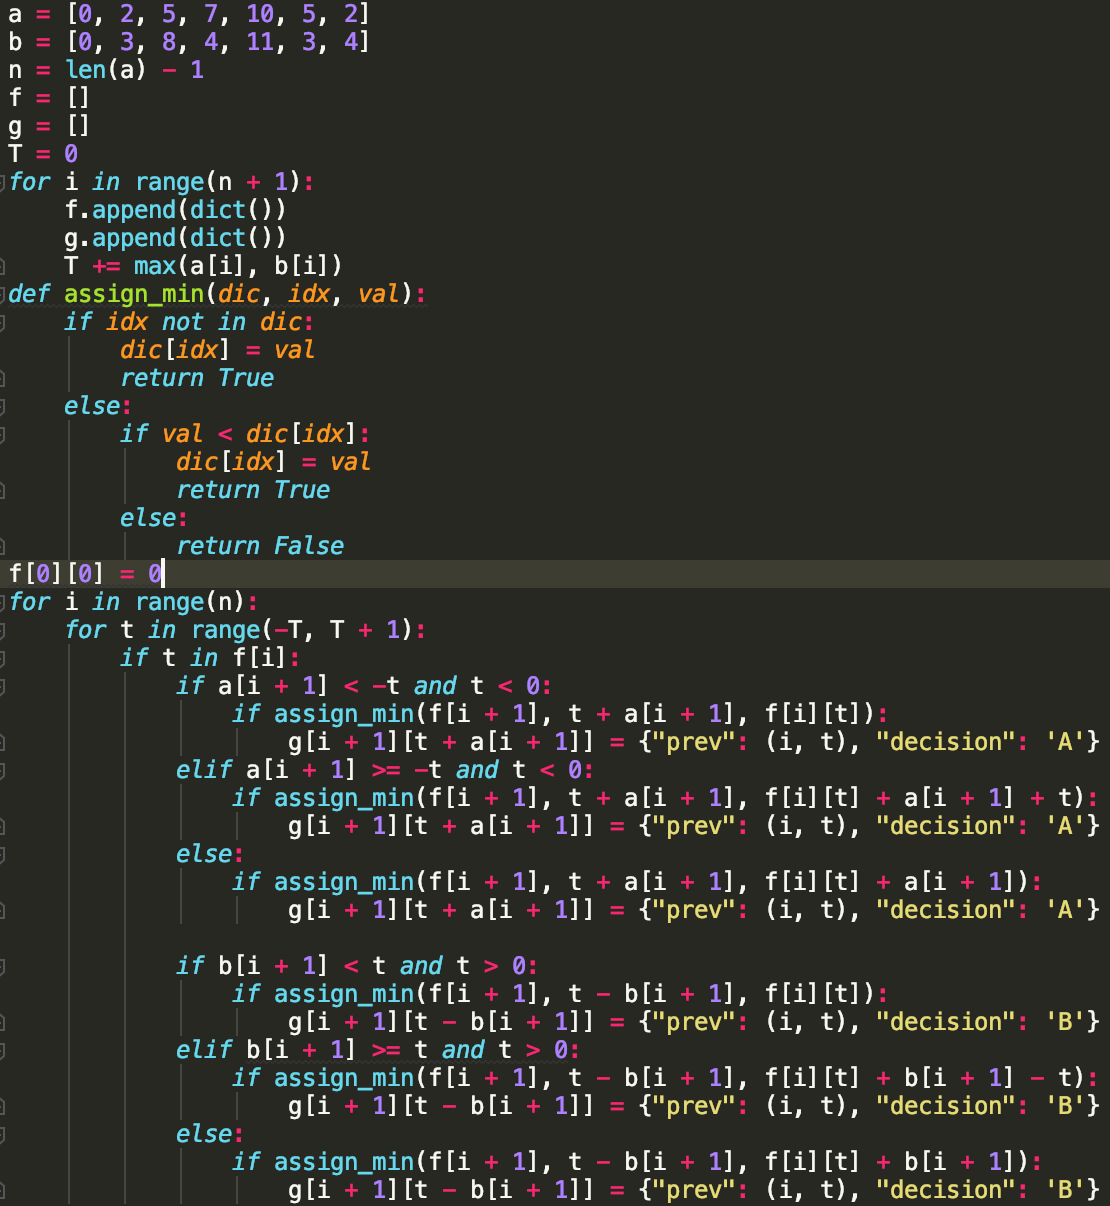
\includegraphics[scale=0.7]{code1.png}
\end{align*}
\begin{align*}
  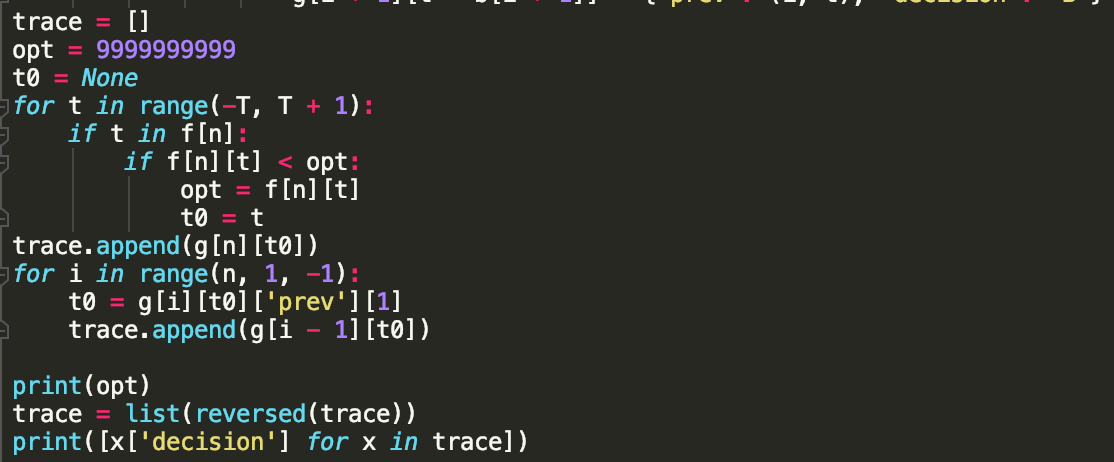
\includegraphics[scale=0.7]{code2.png}
\end{align*} \par
And the result is:
\begin{align*}
  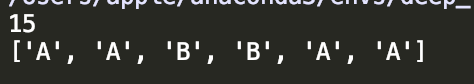
\includegraphics[scale=0.7]{result.png}
\end{align*} \par
So the task 1, 2, 4, 6 should be assigned to A and others should be assigned to B. The total time is 15.
\question{3}
Denote $f[i][j]$ as $\displaystyle\max \displaystyle\sum_{k = 1}^i c_i \cdot x_i$, such that $\displaystyle\sum_{k = 1}^i a_i \cdot x_i \leq j$. \par
Therefore, $f[i][j] = \displaystyle\max_{k \in \{0, 1, 2\} \, and \, k \cdot a[i] \leq j} f[i - 1][j - k * a[i]] + k * c[i]$. Here $ 1 \leq i \leq n$ and $0 \leq j \leq b$. And $f[0][j] = 0$ for $j = 0, 1, ..., b$. The answer required is $f[n][b]$ .Similar to the knapsack problem, the time complexity is $\Theta(min(3^n, nb, n\displaystyle\sum_{i = 1}^n c_i))$.

\question{4}
Denote $f[i][j]$ as the maximum log-reliability after considering the $1, 2, ..., i$-th machine. The dp formula is:
\begin{align}
  f[i][j] = \max_{k \in N \, | \, j - k * c[i] \geq 0} f[i - 1][j - k * c[i]] + ln(g_i(k))
\end{align} \par
The answer required is $e^{f[n][c]}$.
\end{document}
